% !TeX program = lualatex
% このファイルは LuaLaTeX で処理してください(pdfLaTeX/upLaTeXでは動作しません)。
\documentclass[a4paper,11pt]{ltjsarticle}

\usepackage{amsmath,amssymb,mathtools}
\usepackage{siunitx}
\usepackage{geometry}
\geometry{a4paper,top=15mm,bottom=18mm,left=14mm,right=14mm}
\usepackage{tikz}
\usetikzlibrary{arrows.meta,positioning,calc}
\usepackage[most]{tcolorbox}
\usepackage{booktabs}
\usepackage{array}
\usepackage{enumitem}

\setlength{\parindent}{0pt}
\setlength{\parskip}{2pt}
\renewcommand{\arraystretch}{2.6}

\newcommand{\banner}[1]{%
  \begin{tcolorbox}[colback=black,coltext=white,boxrule=0pt,sharp corners,
    left=8pt,right=8pt,top=5pt,bottom=5pt,before skip=8pt,after skip=8pt]
    {\Large\bfseries #1}
  \end{tcolorbox}}

\newcommand{\subbanner}[1]{%
  \begin{tcolorbox}[colback=black!80,coltext=white,boxrule=0pt,sharp corners,
    left=8pt,right=8pt,top=4pt,bottom=4pt,before skip=6pt,after skip=6pt]
    {\large\bfseries #1}
  \end{tcolorbox}}

\newtcolorbox{pointbox}[1][]{%
  colback=black!4,colframe=black,boxrule=0.6pt,arc=1mm,
  left=6pt,right=6pt,top=4pt,bottom=4pt,#1}

\pagestyle{plain}

\begin{document}

\banner{開口端補正 演習}

実際の気柱の振動では，開口端(自由端)にできる腹は，管の口ちょうどの位置ではなく，そこから少し外側にずれた位置にできる。このずれを\textbf{開口端補正}といい，$\Delta x$ で表す(下図の補助的な点線の位置が真の腹の位置。$\Delta x$ の大きさは振動の仕方によらず一定である)。それぞれの図をよく見て，表の空欄をうめよ。音の速さを $V$ とする。

% ------------------------------------------------------
\subbanner{開管の場合（開口端が2か所）}
\noindent\hspace{1.5cm}\begin{tabular}{cc|c|c}
\cline{2-4}

% ---- ヘッダー行 ----
\makebox[3.6cm][l]{\hspace{-1.2cm}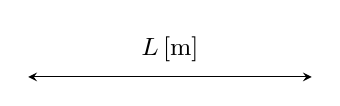
\begin{tikzpicture}[x=1cm,y=1cm]
  \draw[<->,>=stealth] (0,0) -- (3.6,0);
  \node[font=\small] at (1.8,0.35) {$L\,[\mathrm{m}]$};
\end{tikzpicture}}
&
& \textbf{波長 $\lambda\,[\mathrm{m}]$}
& \textbf{振動数 $f\,[\mathrm{Hz}]$} \\
\cline{2-4}

% ---- 基本振動 (n=1)：Δxの矢印を両端に表示 ----
\makebox[3.6cm][l]{\hspace{-1.2cm}\begin{tikzpicture}[x=0.6cm,y=0.6cm]
  \draw[thick] (0,1.3) -- (6,1.3);
  \draw[thick] (0,-1.3) -- (6,-1.3);
  \draw[dashed] (3,2.1) -- (3,-2.1); % 中央の節
  \draw[dotted] (-1,2.1) -- (-1,-2.1); % 補助点線：真の腹（左）
  \draw[dotted] (7,2.1) -- (7,-2.1); % 補助点線：真の腹（右）
  \draw[<->,>=stealth] (-1,1.7) -- (0,1.7); % 開口端補正Δx（左）
  \node[above,font=\tiny] at (-0.5,1.7) {$\Delta x$};
  \draw[<->,>=stealth] (6,1.7) -- (7,1.7); % 開口端補正Δx（右）
  \node[above,font=\tiny] at (6.5,1.7) {$\Delta x$};
\end{tikzpicture}}
& 基本振動 & & \\
\cline{2-4}

% ---- 2倍振動 (n=2) ----
\makebox[3.6cm][l]{\hspace{-1.2cm}\begin{tikzpicture}[x=0.6cm,y=0.6cm]
  \draw[thick] (0,1.3) -- (6,1.3);
  \draw[thick] (0,-1.3) -- (6,-1.3);
  \draw[dashed] (1.5,2.1) -- (1.5,-2.1);
  \draw[dashed] (4.5,2.1) -- (4.5,-2.1);
  \draw[dotted] (-1,2.1) -- (-1,-2.1); % 補助点線：真の腹（左）
  \draw[dotted] (3,2.1) -- (3,-2.1); % 中央（内部）の腹
  \draw[dotted] (7,2.1) -- (7,-2.1); % 補助点線：真の腹（右）
\end{tikzpicture}}
& 2倍振動 & & \\
\cline{2-4}

% ---- 3倍振動 (n=3) ----
\makebox[3.6cm][l]{\hspace{-1.2cm}\begin{tikzpicture}[x=0.6cm,y=0.6cm]
  \draw[thick] (0,1.3) -- (6,1.3);
  \draw[thick] (0,-1.3) -- (6,-1.3);
  \draw[dashed] (1,2.1) -- (1,-2.1);
  \draw[dashed] (3,2.1) -- (3,-2.1);
  \draw[dashed] (5,2.1) -- (5,-2.1);
  \draw[dotted] (-1,2.1) -- (-1,-2.1); % 補助点線：真の腹（左）
  \draw[dotted] (2,2.1) -- (2,-2.1);
  \draw[dotted] (4,2.1) -- (4,-2.1);
  \draw[dotted] (7,2.1) -- (7,-2.1); % 補助点線：真の腹（右）
\end{tikzpicture}}
& 3倍振動 & & \\
\cline{2-4}

% ---- 「以下同様に続く」区切り行 ----
\makebox[3.6cm][l]{\hspace{-1.2cm}\begin{tikzpicture}[x=0.6cm,y=0.6cm]
  \node[font=\small] at (3,0) {$\vdots$};
\end{tikzpicture}}
& $\vdots$ & $\vdots$ & $\vdots$ \\
\cline{2-4}

% ---- n倍振動（一般化） ----
\makebox[3.6cm][l]{\hspace{-1.2cm}\begin{tikzpicture}[x=0.6cm,y=0.6cm]
  \draw[thick] (0,1.3) -- (6,1.3);
  \draw[thick] (0,-1.3) -- (6,-1.3);
  \draw[dotted] (-1,2.1) -- (-1,-2.1); % 補助点線：真の腹（左）
  \draw[dotted] (7,2.1) -- (7,-2.1); % 補助点線：真の腹（右）
  \node[font=\small] at (3,0) {$\cdots$};
\end{tikzpicture}}
& n倍振動 & & \\
\cline{2-4}
\end{tabular}

\clearpage
% -------------------------------------------------------------------
\subbanner{閉管の場合（開口端が1か所）}
\noindent\hspace{1.5cm}\begin{tabular}{cc|c|c}
\cline{2-4}

% ---- ヘッダー行 ----
\makebox[3.6cm][l]{\hspace{-1.2cm}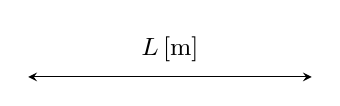
\begin{tikzpicture}[x=1cm,y=1cm]
  \draw[<->,>=stealth] (0,0) -- (3.6,0);
  \node[font=\small] at (1.8,0.35) {$L\,[\mathrm{m}]$};
\end{tikzpicture}}
&
& \textbf{波長 $\lambda\,[\mathrm{m}]$}
& \textbf{振動数 $f\,[\mathrm{Hz}]$} \\
\cline{2-4}

% ---- 基本振動 (m=1)：Δxの矢印を開口端側のみ表示 ----
\makebox[3.6cm][l]{\hspace{-1.2cm}\begin{tikzpicture}[x=0.6cm,y=0.6cm]
  \fill[black] (-0.08,-1.3) rectangle (0,1.3); % 閉端（固定壁）
  \draw[thick] (0,1.3) -- (6,1.3);
  \draw[thick] (0,-1.3) -- (6,-1.3);
  \draw[dotted] (7,2.1) -- (7,-2.1); % 補助点線：真の腹（開口端側）
  \draw[<->,>=stealth] (6,1.7) -- (7,1.7); % 開口端補正Δx
  \node[above,font=\tiny] at (6.5,1.7) {$\Delta x$};
\end{tikzpicture}}
& 基本振動 & & \\
\cline{2-4}

% ---- 3倍振動 (m=3) ----
\makebox[3.6cm][l]{\hspace{-1.2cm}\begin{tikzpicture}[x=0.6cm,y=0.6cm]
  \fill[black] (-0.08,-1.3) rectangle (0,1.3);
  \draw[thick] (0,1.3) -- (6,1.3);
  \draw[thick] (0,-1.3) -- (6,-1.3);
  \draw[dashed] (4,2.1) -- (4,-2.1);
  \draw[dotted] (2,2.1) -- (2,-2.1);
  \draw[dotted] (7,2.1) -- (7,-2.1); % 補助点線：真の腹（開口端側）
\end{tikzpicture}}
& 3倍振動 & & \\
\cline{2-4}

% ---- 5倍振動 (m=5) ----
\makebox[3.6cm][l]{\hspace{-1.2cm}\begin{tikzpicture}[x=0.6cm,y=0.6cm]
  \fill[black] (-0.08,-1.3) rectangle (0,1.3);
  \draw[thick] (0,1.3) -- (6,1.3);
  \draw[thick] (0,-1.3) -- (6,-1.3);
  \draw[dashed] (2.4,2.1) -- (2.4,-2.1);
  \draw[dashed] (4.8,2.1) -- (4.8,-2.1);
  \draw[dotted] (1.2,2.1) -- (1.2,-2.1);
  \draw[dotted] (3.6,2.1) -- (3.6,-2.1);
  \draw[dotted] (7,2.1) -- (7,-2.1); % 補助点線：真の腹（開口端側）
\end{tikzpicture}}
& 5倍振動 & & \\
\cline{2-4}

% ---- 「以下同様に続く」区切り行 ----
\makebox[3.6cm][l]{\hspace{-1.2cm}\begin{tikzpicture}[x=0.6cm,y=0.6cm]
  \node[font=\small] at (3,0) {$\vdots$};
\end{tikzpicture}}
& $\vdots$ & $\vdots$ & $\vdots$ \\
\cline{2-4}

% ---- (2n-1)倍振動（一般化） ----
\makebox[3.6cm][l]{\hspace{-1.2cm}\begin{tikzpicture}[x=0.6cm,y=0.6cm]
  \fill[black] (-0.08,-1.3) rectangle (0,1.3);
  \draw[thick] (0,1.3) -- (6,1.3);
  \draw[thick] (0,-1.3) -- (6,-1.3);
  \draw[dotted] (7,2.1) -- (7,-2.1); % 補助点線：真の腹（開口端側）
  \node[font=\small] at (3.333,0) {$\cdots$};
\end{tikzpicture}}
& $(2n-1)$倍振動 & & \\
\cline{2-4}
\end{tabular}

\begin{pointbox}
\textbf{ヒント}：管口ちょうどではなく，補助の点線の位置(管口から $\Delta x$ だけ外側)に腹ができるものとして図を読む。あとは，これまでと同じように「節と節（または腹と腹）の間隔は $\lambda/2$」に着目し，実際の管の長さ $L$ に開口端補正 $\Delta x$ を加えた長さが波長 $\lambda$ の何倍にあたるかを考えればよい。求めた $\lambda$ から $f=\dfrac{V}{\lambda}$ で振動数も求まる。
\end{pointbox}

\end{document}
